%TeX 
% Gemini theme
% https://github.com/anishathalye/gemini
%
% We try to keep this Overleaf template in sync with the canonical source on
% GitHub, but it's recommended that you obtain the template directly from
% GitHub to ensure that you are using the latest version.

\documentclass[aspectratio=32, final]{beamer}

% ====================
% Packages
% ====================

\usepackage[T1]{fontenc}
\usepackage{lmodern}
\usepackage[size=custom,width=120,height=80,scale=1.0]{beamerposter}
\usetheme{gemini}
\usecolortheme{gemini}
\usepackage{graphicx}
\usepackage{booktabs}
\usepackage{tikz}
\usepackage{pgfplots}
\usepackage{svg}
\usepackage{multicol}

% ====================
% Lengths
% ====================

% If you have N columns, choose \sepwidth and \colwidth such that
% (N+1)*\sepwidth + N*\colwidth = \paperwidth
\newlength{\sepwidth}
\newlength{\colwidth}
\setlength{\sepwidth}{0.025\paperwidth}
\setlength{\colwidth}{0.3\paperwidth}

\newcommand{\separatorcolumn}{\begin{column}{\sepwidth}\end{column}}

% ====================
% Title
% ====================

\title{Catastrophic Forgetting versus Model Robustness in BNNs}

\author{Tuan Pham \and Amit Pradhan \and Sebastian Barrios}

\institute[shortinst]{\{tuanph18, pradhanak, sbarrios\}@uchicago.edu}

% ====================
% Body
% ====================

\begin{document}

\begin{frame}[t]
\begin{columns}[t]
\separatorcolumn

\begin{column}{0.58\colwidth}

  \begin{block}{Motivation}

    A recent study \cite{Laborieux2021-pv} takes inspiration from biological metaplasticity to solve catastrophic forgetting (CF) problems and continual learning problems for binary neural networks (BNN). More specifically, by creating a form of multiplicative gating during learning for hidden weights to represent weight consolidation, they are able to solve the permuted-MNIST task, sequential learning with CIFAR-10/100 dataset, and stream learning with these datasets. The metaplasticity method shows promise of reduced precision models in continual learning context. However, quantized neural networks are also known to be sensitive to input perturbation \cite{Lin2019-xs}, specifically adversarial attacks \cite{Goodfellow2014-bu}. This poses a question on whether binary networks trained to prevent catastrophic forgetting would generally be sensitive or robust towards different types of input perturbation, particularly natural corruptions \cite{Hendrycks2018-ae} and adversarial attacks. 

  \end{block}

  \begin{alertblock}{Binary Neural Networks (BNN)}

    An attractive solution for fast computation, efficient power consumption and potentially easier hardware implementation is BNN, in which only the signs of the model’s hidden weights are utilized during inference. 
    
    \begin{figure}
        \centering
        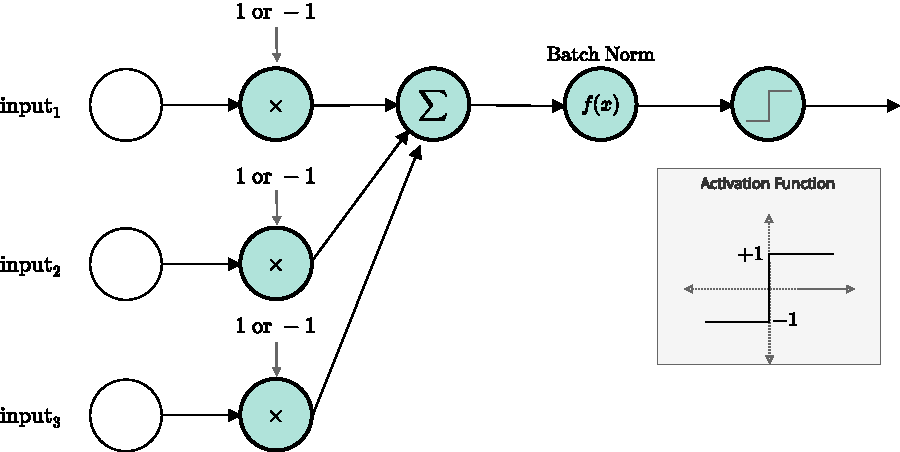
\includegraphics[width=0.5\colwidth]{figures/bnn.pdf}
    \end{figure}
    
  \end{alertblock}
  
  \begin{block}{Synaptic Metaplasticity \cite{Laborieux2021-pv} }
 

 \begin{figure}
     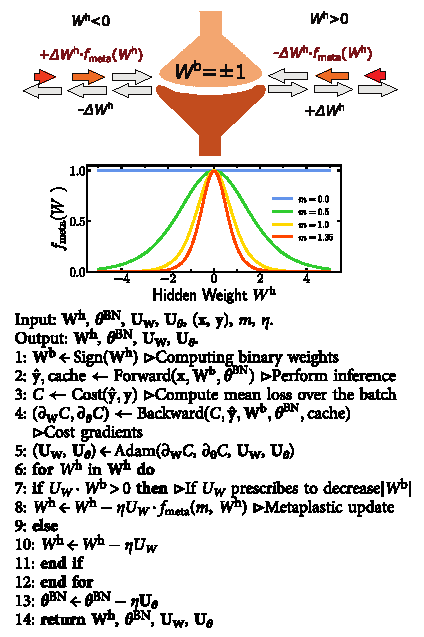
\includegraphics[width=0.42\colwidth]{figures/metaplasticity.pdf}
 \end{figure}
 
\end{block}

\end{column}

\separatorcolumn

\begin{column}{1.2\colwidth}
    
  \begin{block}{Permuted MNIST reproducibility}
    
    The values of \texttt{meta} show the effects similar to the paper: increased \texttt{meta} allows to prevent catastrophic forgetting for pMNIST task in a 2-layer MLP. However, the size effects were not reproducible as increased in size is counter-effective. 
    
    \begin{figure}
        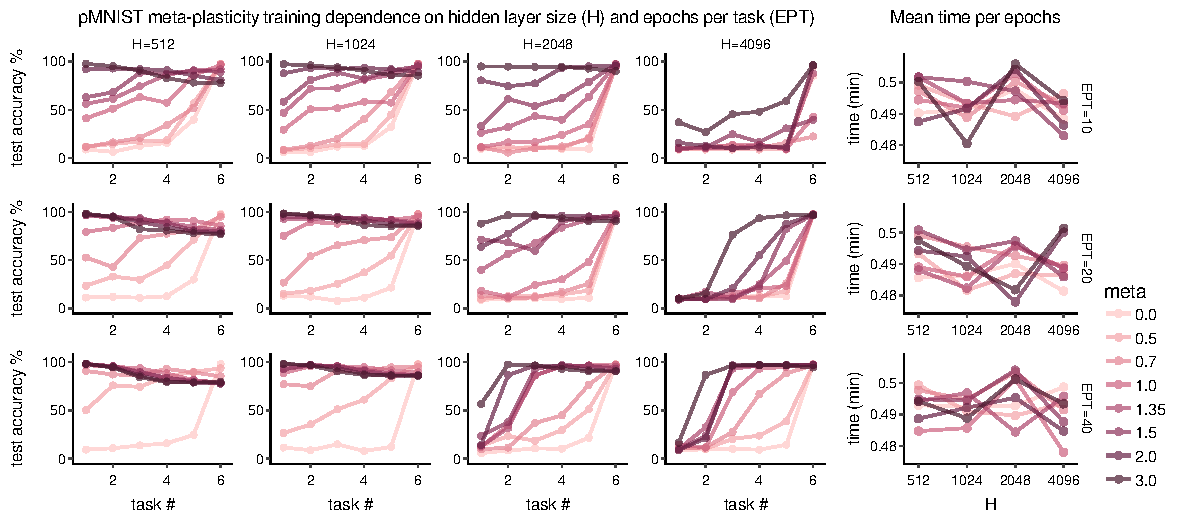
\includegraphics[width=1.2\colwidth]{figures/reproduce.pdf}
    \end{figure}
  \end{block}

  \begin{block}{pMNIST - Robustness}
  
    \textbf{Lipschitz regularization - Defensive quantization} \cite{Lin2019-xs}: $\frac{1}{2}\beta_{\mathrm{DQ}}\sum \lVert \mathbf{W}^T\mathbf{W} - \mathbf{I} \rVert^2$
    
    \begin{figure}
        \centering
        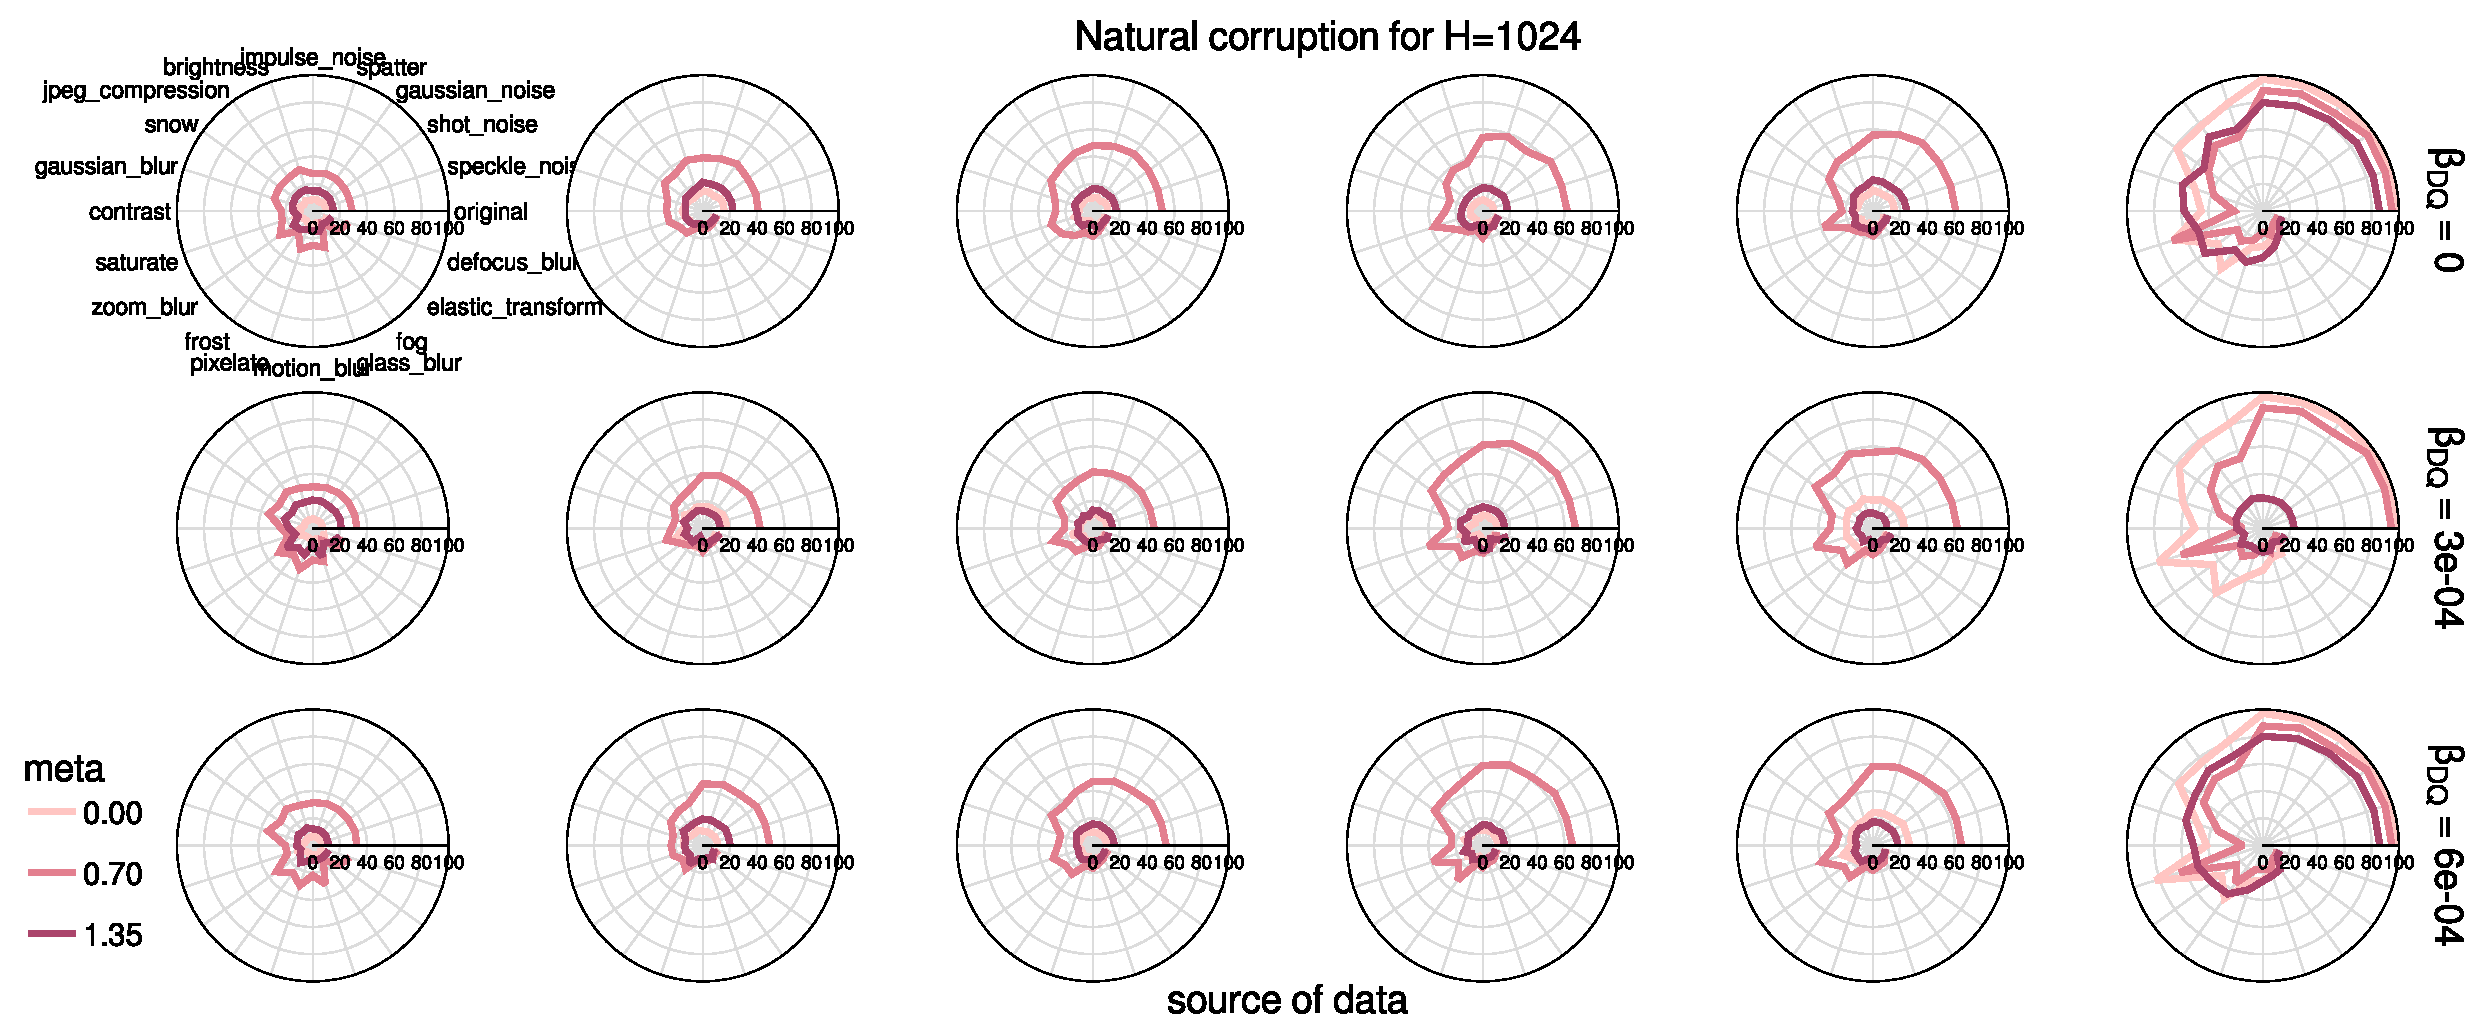
\includegraphics[width=1.2\colwidth]{figures/vary-meta-dq-natcrpt-H=1024.pdf}
    \end{figure}

    \begin{figure}
        \centering
        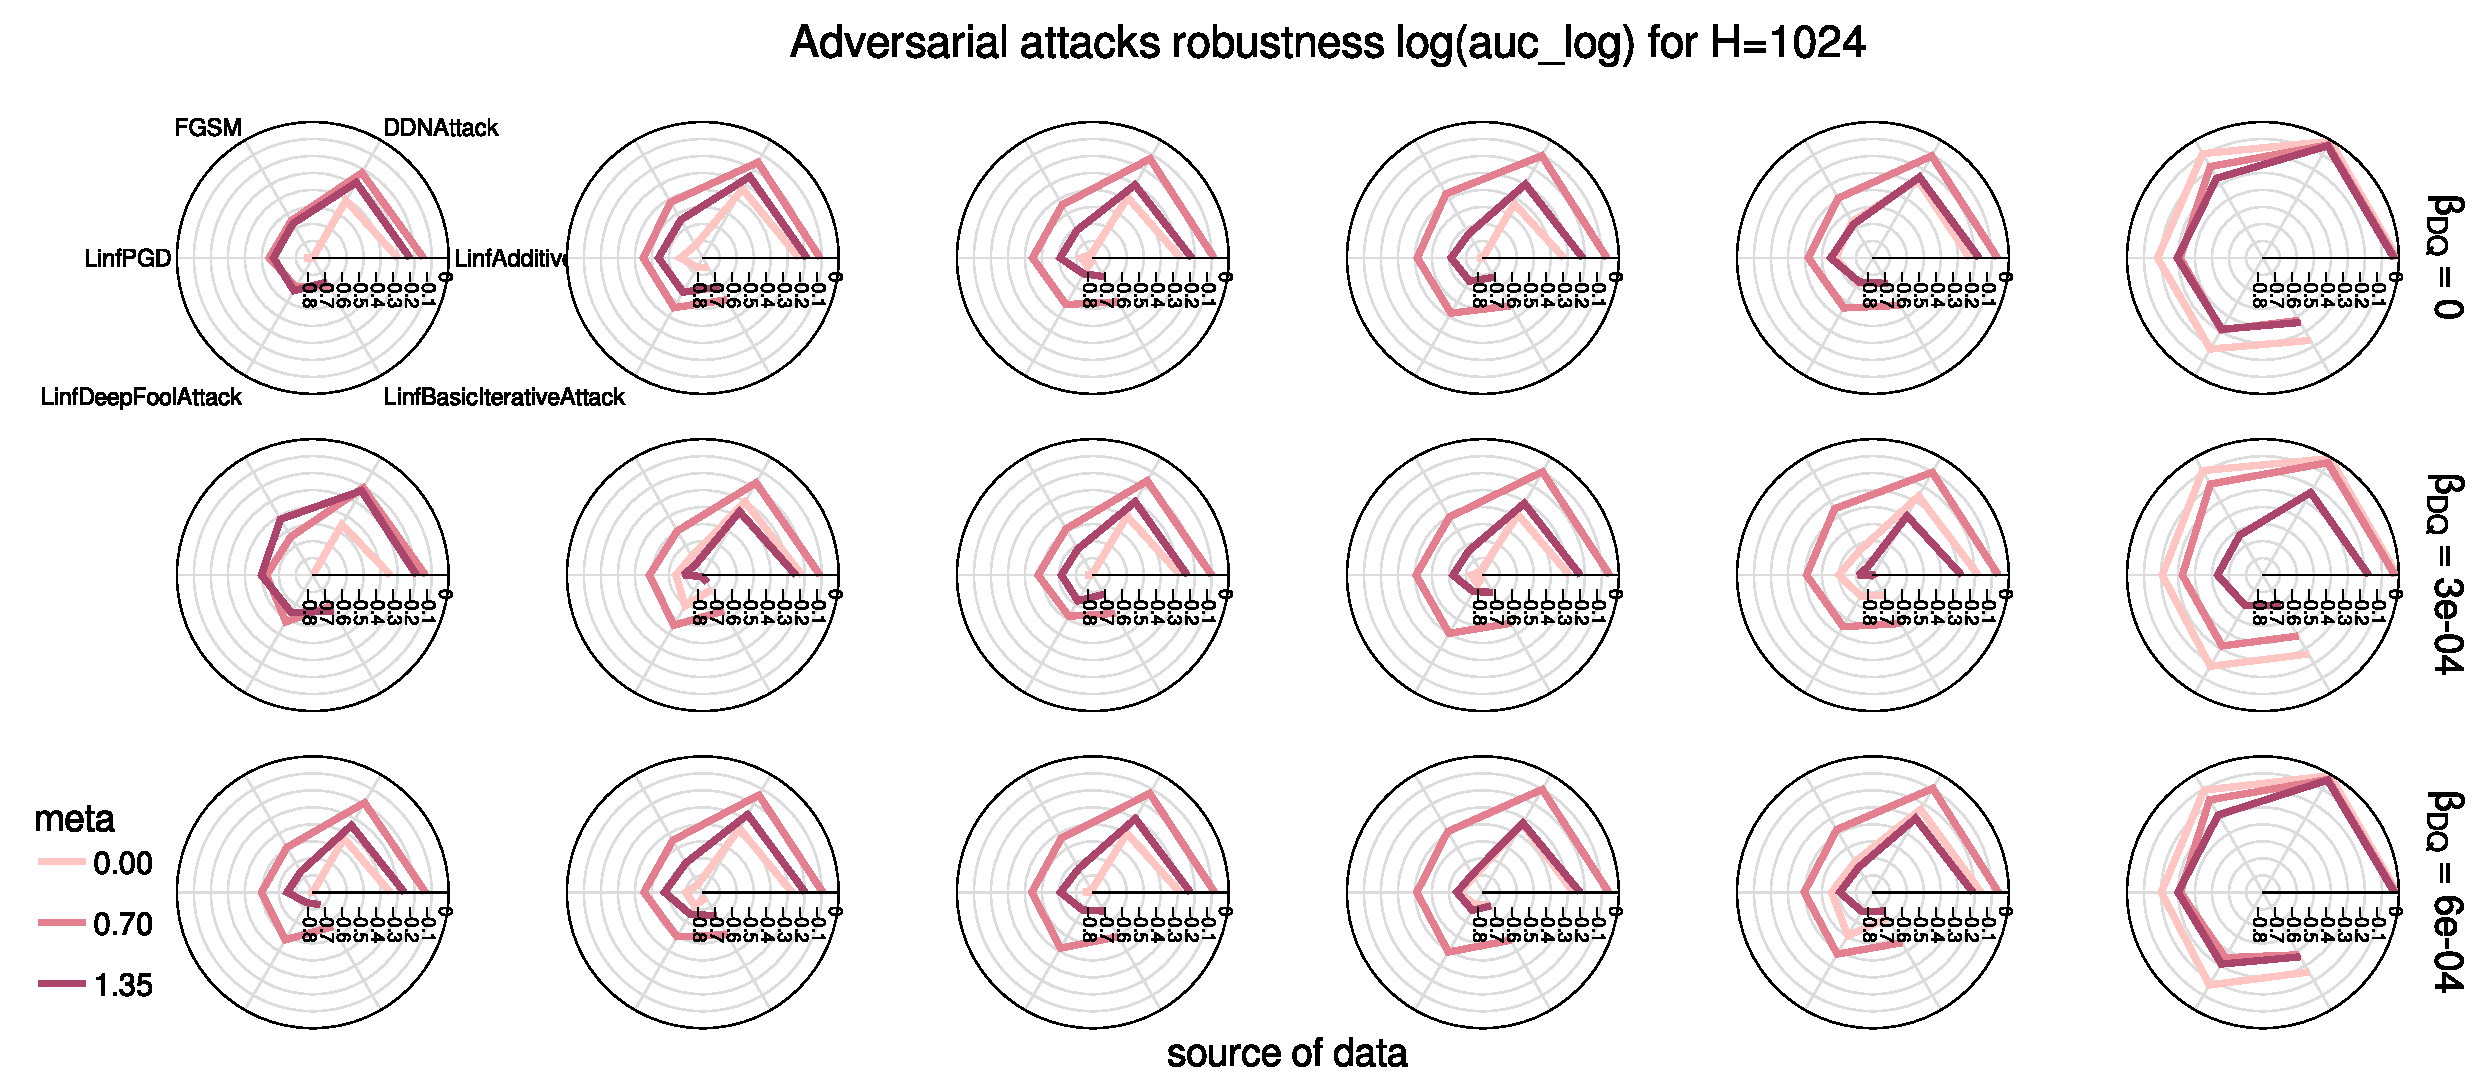
\includegraphics[width=1.2\colwidth]{figures/vary-meta-dq-advatck-auc_log-H=1024.pdf}
    \end{figure}
    
  \end{block}

\end{column}

\separatorcolumn

\begin{column}{1.1\colwidth}

  \begin{block}{CIFAR split-class}
  
  \begin{figure}
      \centering
      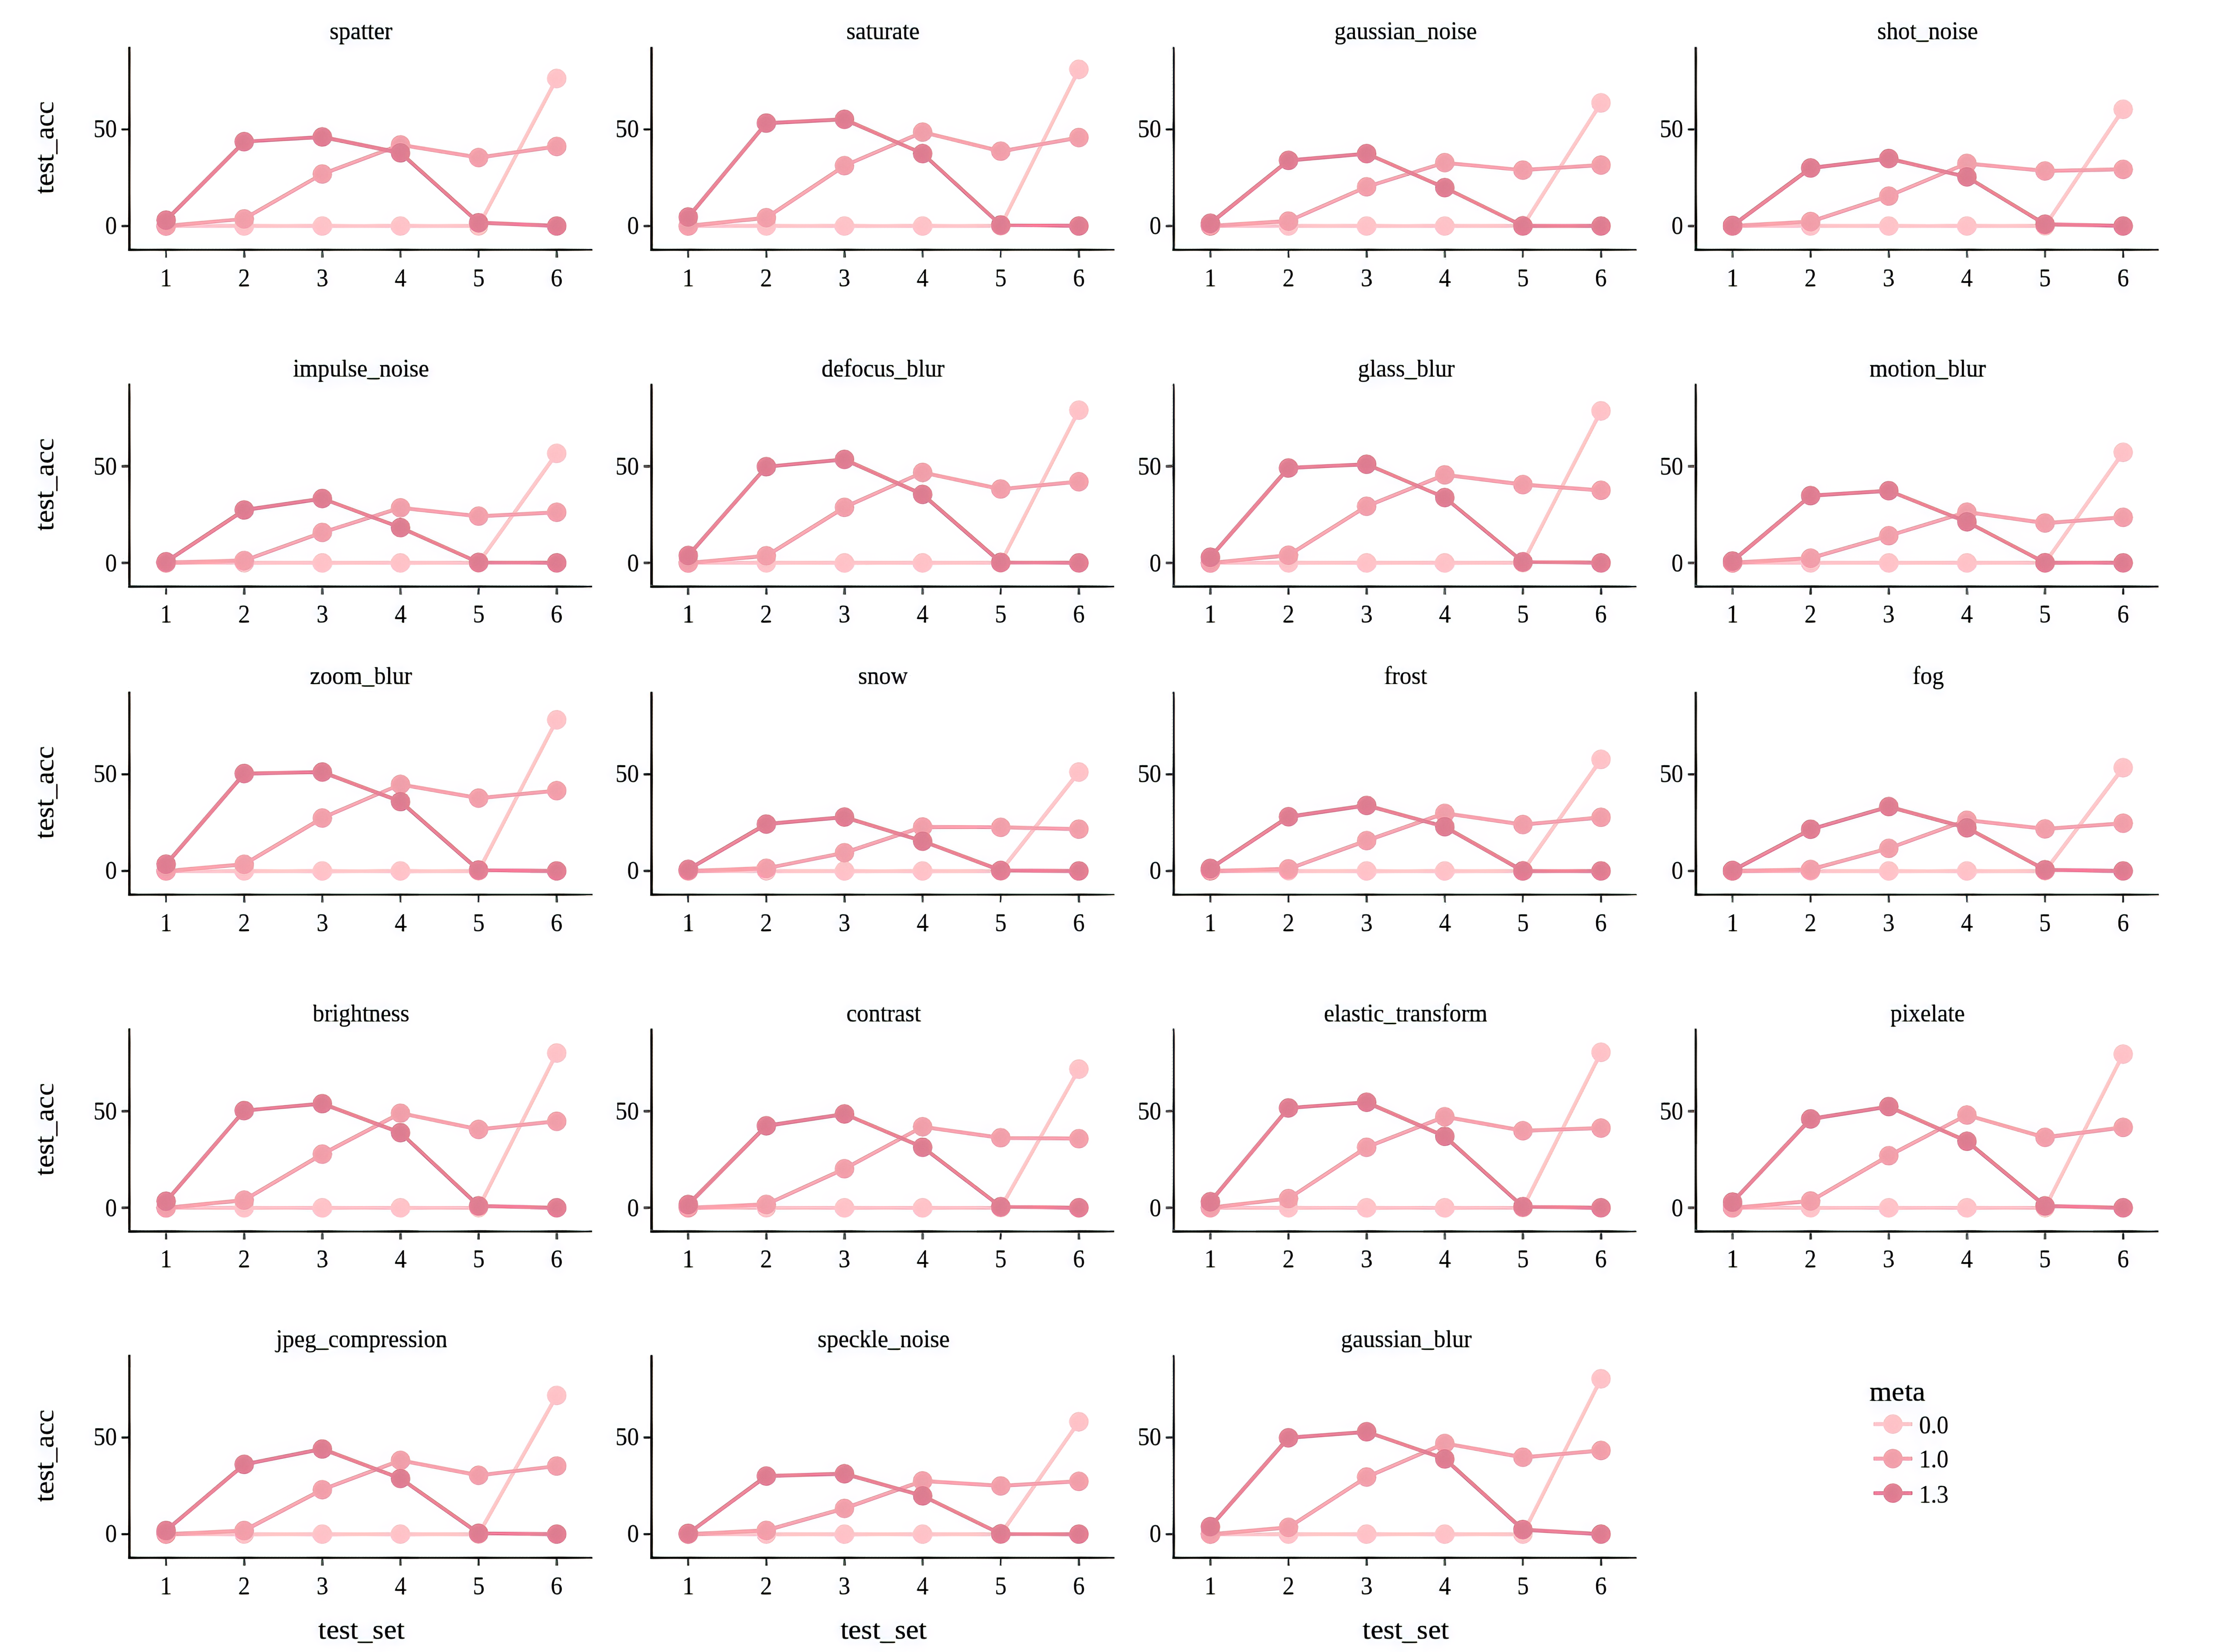
\includegraphics[width=1.0\colwidth]{figures/corruption_cifar100.png}
  \end{figure}

    \begin{figure}
      \centering
      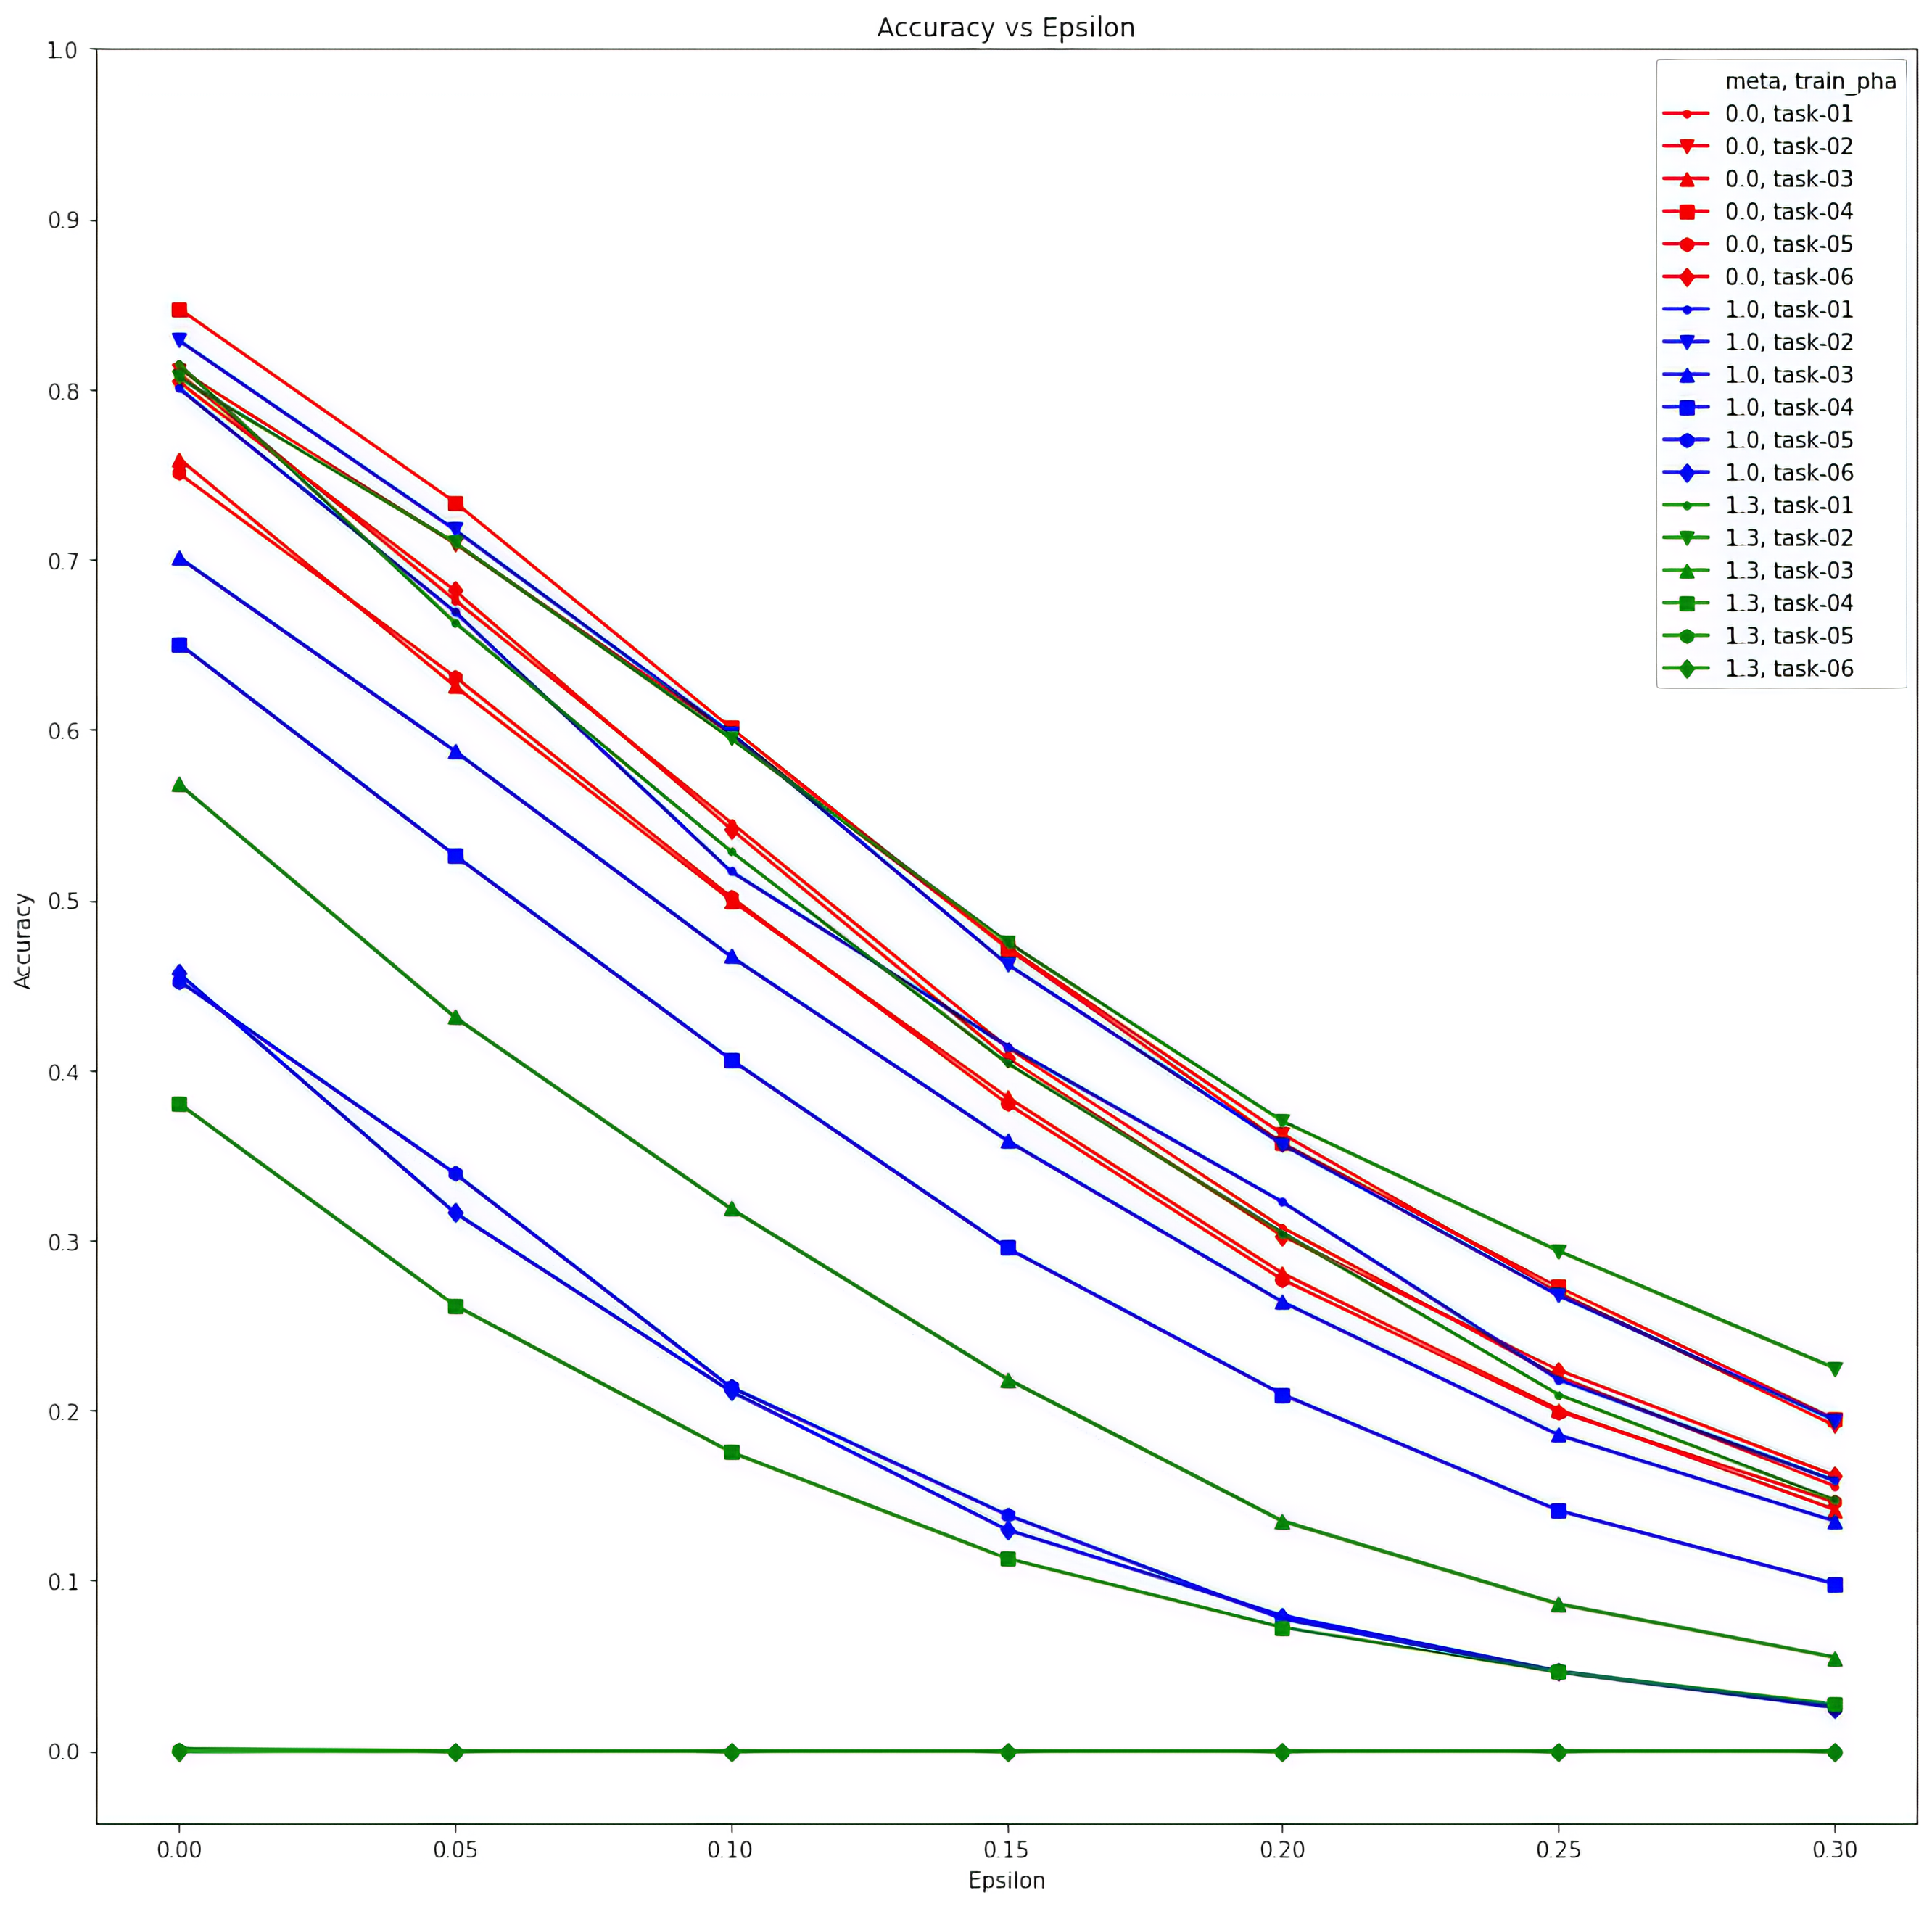
\includegraphics[width=0.5\colwidth]{figures/cifar100-fgsm-attack.png}
  \end{figure}
  \end{block}

  \begin{block}{Conclusions}
    While metaplasticity for BNN was useful to prevent catastrophic forgetting (pMNIST and split-class CIFAR tasks), the resulting models were not as robust. There appears to be a trade-off for continual learning and robustness - only medium values of \texttt{meta} would result in more robust models. Additionally, for the pMNIST task, Lipschitz regularization has mixed effects on model robustness for attacks and corruptions, for the pMNIST task.
    
    However, there were also issues within the metaplasticity training: (1) dependence on the task-relevant batchnorm states, (2) irreproducible network size benefits as seen in the paper \cite{Laborieux2021-pv}. Plus, we did not have time to assess model compression benefits and speed in comparison with real-valued networks - one reason was the fact that metaplasticity was not effective in such networks. However, future experiments could involve (1) more continual learning tasks, (2) more systematic comparisons (performance, time, inference, memory cost, robustness) between different known solutions for catastrophic forgetting for neural networks across different quantization levels.
    

    \tiny{
        \bibliographystyle{ieeetr}
        \bibliography{poster}
    }
  \end{block}

  




\end{column}

\separatorcolumn



\end{columns}

\end{frame}

\end{document}
